% Created 2022-08-31 mié 09:01
% Intended LaTeX compiler: pdflatex
\documentclass[12pt]{article}
\usepackage[utf8]{inputenc}
\usepackage[T1]{fontenc}
\usepackage{graphicx}
\usepackage{grffile}
\usepackage{longtable}
\usepackage{wrapfig}
\usepackage{rotating}
\usepackage[normalem]{ulem}
\usepackage{amsmath}
\usepackage{textcomp}
\usepackage{amssymb}
\usepackage{capt-of}
\usepackage{hyperref}
\usepackage[spanish]{babel}
\usepackage{graphicx,geometry}
\geometry{ a4paper, left=1in, right=1in, top=1in, bottom=1in }
\renewcommand\familydefault{\sfdefault}
\usepackage{sectsty}
\sectionfont{\normalfont\Large }
\subsectionfont{\normalfont}
\usepackage{tabularx}
\usepackage{listings}
\lstdefinestyle{mystyle}{
numbers=left,
showspaces=false,
frame=leftline,
showspaces=false,
showstringspaces=false,
showtabs=false,
numberstyle=\tiny,
}
\lstset{
style=mystyle,
literate={á}{{\'a}}1
{é}{{\'e}}1
{í}{{\'{\i}}}1
{ó}{{\'o}}1
{ú}{{\'u}}1
{Á}{{\'A}}1
{É}{{\'E}}1
{Í}{{\'I}}1
{Ó}{{\'O}}1
{Ú}{{\'U}}1
{ü}{{\"u}}1
{Ü}{{\"U}}1
{ñ}{{\~n}}1
{Ñ}{{\~N}}1
{¿}{{?``}}1
{¡}{{!``}}1
}
\makeatletter
\usepackage{fancyhdr}
\pagestyle{fancy}
\usepackage{mdframed}
\BeforeBeginEnvironment{minted}{\begin{mdframed}}
\AfterEndEnvironment{minted}{\end{mdframed}}
\author{Luis Eduardo Galindo Amaya \\
1274895}
\date{2022-08-29}
\title{Interconexión de Elementos en la Organización de una Computadora de Propósito General}
\hypersetup{
 pdfauthor={Luis Eduardo Galindo Amaya \\
1274895},
 pdftitle={Interconexión de Elementos en la Organización de una Computadora de Propósito General},
 pdfkeywords={},
 pdfsubject={},
 pdfcreator={Emacs 26.3 (Org mode 9.1.9)}, 
 pdflang={Spanish}}
\begin{document}



\newcommand{\docente}{Arturo Arreola Alvarez}
\newcommand{\asignatura}{Organización de Computadoras (331)}
\newcommand{\semestre}{2022-2}

\newcommand{\miportada}[1]{
	\begin{titlepage}
		\vspace*{0.75in}
		\begin{flushleft}
			\sffamily
			\large #1       \\
			\Huge 
            \@title         \\
			\hrulefill
			\vspace{0.25in} \\
			\Large \@author \\
			\vspace*{\fill}
            
\includegraphics[width=\textwidth]{../includes/filler.png} \\
			\vspace*{\fill}
			\large
			\begin{tabular}{|l|l|}
              \hline
			  Asignatura & \asignatura \\
			  Docente    & \docente    \\
			  Fecha      & \@date      \\
              \hline
			\end{tabular}
		\end{flushleft}
	\end{titlepage}
}

\miportada{ Práctica 2 }

\fancyhf{}
\lhead{ \asignatura }
\rhead{ \semestre }
\rfoot{Página \thepage}

\setlength\parindent{0pt}   % eliminar el intentado
\setlength{\parskip}{1.2em}
\maketitle

\section*{Cuestionario}
\label{sec:org7ae24a0}
\begin{enumerate}
\item ¿Qué tamaño en bits tiene el bus de direcciones?
\begin{itemize}
\item 12 bits.
\end{itemize}

\item ¿Qué tamaño en bits tiene el bus de datos?
\begin{itemize}
\item 16 bits.
\end{itemize}

\item ¿Qué tamaño en bits tiene el código de operación (opcode) de las instrucciones?
\begin{itemize}
\item 16 bits\footnote{Los primeros 4 bits son para la intruccion y los siguientes 12 son para representar direcciones.\label{org5c1096b}}.
\end{itemize}

\item ¿Cuál es la dirección máxima de memoria que se puede acceder?
\begin{itemize}
\item El bus de memoria es solo de 12 bits por lo que la maxima posicion de memoria accesibles es \(2^12 = 4096\) bits\footnote{1000 en hexadecimal. En la linea 65 en \href{https://github.com/MARIE-js/MARIE.js/blob/master/src/js/marie.js}{código} de marie.js esta explícitamente definido.}.
\end{itemize}

\item ¿Por qué el registro \texttt{MAR} es de 12 bits?
\begin{itemize}
\item \texttt{MAR} es el acronimo de "Memory Address Register" y sirve para acumular la posicion memoria que se vaya a operar, por lo tanto esta conectada al bus de direcciones, y el bus de direcciones es de 12 bits \textsuperscript{\ref{org5c1096b}}.
\end{itemize}

\item ¿Por qué el registro \texttt{MBR} es de 16 bits?
\begin{itemize}
\item El \texttt{MBR} esta conectado al bus de datos y solo contiene el valor del buffer de datos,
\end{itemize}
\end{enumerate}

\section*{Programa: Lista de Arrays}
\label{sec:org67a5676}
\lstinputlisting{src/lista-con-punteros.mas}

\subsection*{Capturas}
\label{sec:org8c142ed}
\begin{figure}[htbp]
\centering
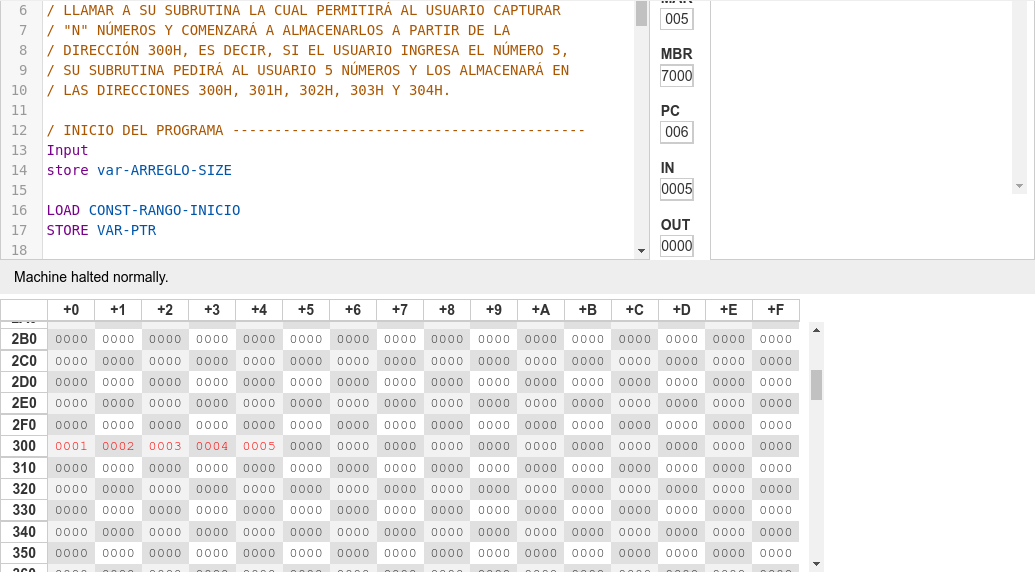
\includegraphics[width=12cm]{./img/capturaArreglo.png}
\caption{Captura de 5 valores, en color rojo.}
\end{figure}

\pagebreak

\section*{Programa: Área Del Triangulo}
\label{sec:org64eb337}
\lstinputlisting{src/area-de-un-triangulo.mas}

\subsection*{Captura}
\label{sec:orgbd9bb05}
\begin{figure}[htbp]
\centering
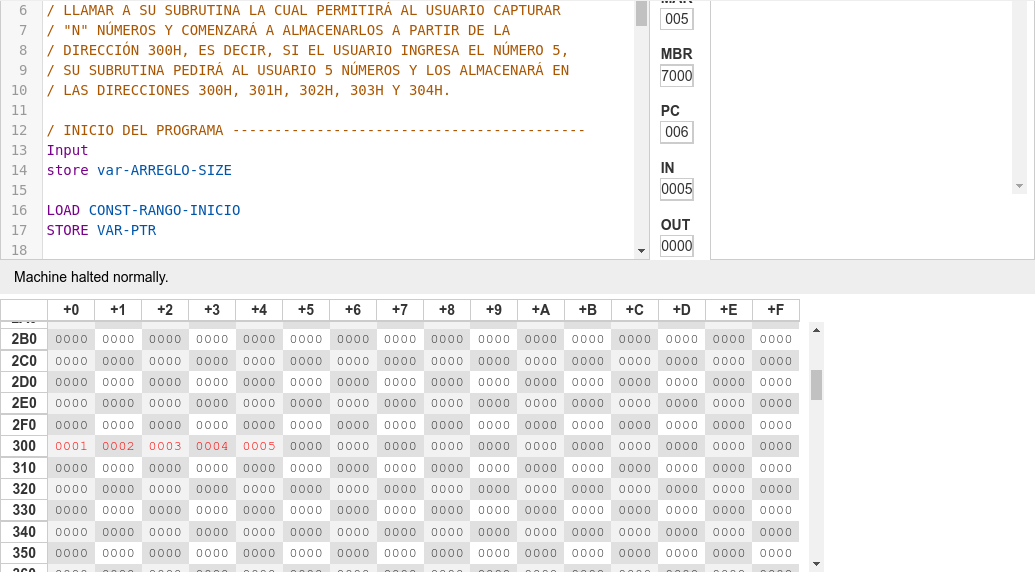
\includegraphics[width=10cm]{./img/capturaArreglo.png}
\caption{Con base 10, altura 5.}
\end{figure}

\section*{Conclusión}
\label{sec:org8c2fde4}
\begin{mdframed}
A modo de conclusión me gustaría poner mis reflexiones, Al tener operaciones muy limitadas en marie.js es muy complicado de obtener el valor de una división, se tiene que recurrir a métodos mas sencillos para poder realizar las operaciones más complejas, recuerdo que algunos profesores siempre nos dicen: \emph{"Las computadoras son tontas"} y al programar en assembly, recuerdo lo sencillas que realmente son es nuestro trabajo como programadores expandir las limitadas capacidades de estos dispositivos para que sean realmente útiles.
\end{mdframed}
\end{document}
